% LaTeX fixture for generating earthquake exposure information

% Standard document class set to landscape
\documentclass[a4paper]{article}

% Extra packages
\usepackage[hmargin=3mm,vmargin=10mm]{geometry}
\usepackage[usenames,dvipsnames]{color}
\usepackage{graphicx}
\usepackage{courier}
\usepackage{colortbl}

% Define background colours for MMI levels
\definecolor{I}{RGB}{0,0,255}
\definecolor{II}{RGB}{32,159,255}
\definecolor{III}{RGB}{0,207,255}
\definecolor{IV}{RGB}{85,255,255}
\definecolor{V}{RGB}{170,255,255}
\definecolor{VI}{RGB}{255,240,0}
\definecolor{VII}{RGB}{255,168,0}
\definecolor{VIII}{RGB}{255,112,0}
\definecolor{IX}{RGB}{255,0,0}
\definecolor{X}{RGB}{240,0,240}

% Fixed width coloured cell
% Usage: \cell{color}{text}
\newcommand{\cell}[2]{
  \cellcolor{#1}
  \makebox[1.3cm]{#2}
}

% No page numbering
\pagestyle{empty}

% Begin document in earnest
\begin{document}

% Header
\begin{tabular}{lcr}
    
\includegraphics[width=0.08\textwidth]{bnpb_logo} &
    \raisebox{10mm}{\parbox{0.75\textwidth}{\Huge \centerline{\textbf{Perkiraan Dampak Gempa}}}} &
    
\includegraphics[width=0.08\textwidth]{bmkg_logo}
\end{tabular}


% Earthquake statistics as per BMKG sms
\bigskip
\input{event_statistics.tex}

% MMI legend
\bigskip
\input{exposure_table.tex}

% Map elements
\bigskip
\begin{tabular}{@{}l@{}l}
  \Large \textbf{Penduduk Paparan} & \\
  \parbox[t]{0.7\textwidth}{
    \vspace{0pt}
    \includegraphics{exposure_map}} &
  \hspace{-8mm}
  \parbox[t]{0.3\textwidth}{
    %\vspace{0pt}
    \vspace{2mm}
    \includegraphics[angle=270,width=0.3\textwidth]{city_legend} \\
    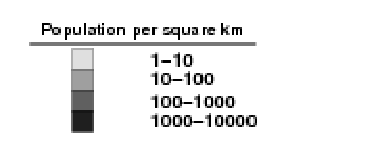
\includegraphics{population_legend}\\
    \includegraphics[width=0.3\textwidth]{mini_map}
  }
\end{tabular}


\end{document}

% PAGE 2
%% \clearpage
%% % Header
%% \begin{tabular}{lcr}
    
\includegraphics[width=0.08\textwidth]{bnpb_logo} &
    \raisebox{10mm}{\parbox{0.75\textwidth}{\Huge \centerline{\textbf{Perkiraan Dampak Gempa}}}} &
    
\includegraphics[width=0.08\textwidth]{bmkg_logo}
\end{tabular}


%% % Earthquake statistics as per BMKG sms
%% \bigskip
%% \input{event_statistics.tex}

%% % MMI legend
%% \bigskip
%% \includegraphics[angle=270,width=1.0\textwidth]{exposure_legend} \\

%% % Map elements
%% \bigskip
%% \begin{tabular}{l@{}l}
%%   \Large \textbf{Penduduk Paparan} & \\
%%   \parbox[t]{0.7\textwidth}{
%%     \vspace{0pt}
%%     \includegraphics{exposure_map}} &
%%   \parbox[t]{0.3\textwidth}{
%%     \vspace{0pt}
%%     \includegraphics[angle=270,width=0.25\textwidth]{city_legend} \\
%%     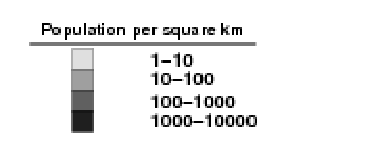
\includegraphics{population_legend}\\
%%     \includegraphics[width=0.25\textwidth]{mini_map}
%%   }
%% \end{tabular}


%% \end{document}


